%==============================================================================
% presentation.tex
%==============================================================================


%==============================================================================
% Configuration
%==============================================================================

% Internationalisation
\usepackage[utf8]{inputenc}
\usepackage[T1]{fontenc}
% \usepackage[ngerman]{babel}

% Different packages
\usepackage{url}
\usepackage{color,listings,paralist}
\usepackage{enumerate}
\usepackage{tabularx}
\usepackage{alltt}

% Use default Acrobat reader fonts
\usepackage{mathpazo}

% Use CM fonts (increases document size)
\usepackage{ae}

% Use images
\usepackage{graphicx}

% Configure beamer
\usetheme[secheader]{Ikhono}
\usefonttheme[onlylarge]{structurebold}
\setbeamertemplate{navigation symbols}{}

% Variables
\providecommand{\Title}{Parallel Programming}
\providecommand{\Subtitle}{Recitation Session 9}
\providecommand{\Author}{Thomas Weibel <weibelt@ethz.ch>}
\providecommand{\Institute}{Laboratory for Software Technology, \\
  Swiss Federal Institute of Technology Z\"urich}
\providecommand{\Date}{May 6, 2010}

% PDF settings
\hypersetup{
  pdftitle={\Title, \Subtitle},
  pdfauthor={\Author},
  pdfsubject={\Institute},
  pdfkeywords={parallel programming} 
}

% Titlepage
\title{\Title}
\subtitle{\Subtitle}
\author{\Author}
\institute{\Institute}
\date{\Date}

% Listings
\lstdefinestyle{Default}{
  language=Java,
  tabsize=2,
  mathescape=true,
  inputencoding=utf8,
  showstringspaces=false,
  fontadjust=true,
  basicstyle=\ttfamily,
  keywordstyle=\color{blue}\bfseries,
}
\lstset{style=Default}


%==============================================================================
% Document
%==============================================================================

\begin{document}


% Titlepage
\begin{frame}[plain]
  \titlepage
\end{frame}


\section*{Introduction}

\begin{frame}{Executive Summary}
  \begin{itemize}
  \item Lack of fairness when using monitors
    \begin{itemize}
    \item Alternatives when we have to guarantee fairness
    \end{itemize}
  \item JCSP: Classroom exercises
  \item MergeSort implementation using JCSP
  \item Swing and the Model-View-Controller pattern
  \item Conway's Game of Life
  \end{itemize}
\end{frame}


\section{Fairness}

\begin{frame}{Outline}
  \tableofcontents[current]
\end{frame}

\begin{frame}[fragile]{Monitors}
\begin{lstlisting}
public class Synchronizer {
  public synchronized void doSynchronized() {
    //do a lot of work which takes a long time
  }
}
\end{lstlisting}

  \vspace{\stretch{1}}

  \begin{alertblock}{No fairness!}
    \begin{itemize}
    \item If more than one thread call the
      \lstinline!doSynchronized()!  method, some of them will be
      blocked until the first thread granted access has left the
      method
    \item If more than one thread are blocked waiting for access there
      is no guarantee about which thread is granted access next
    \end{itemize}
  \end{alertblock}
\end{frame}

\begin{frame}[fragile]{\lstinline!wait()!}
  \begin{itemize}
  \item Causes the current thread to wait until another thread invokes
    the \lstinline!notify()! method or the \lstinline!notifyAll()!
    method for this object
  \item A thread can also wake up without being notified, interrupted,
    or timing out: \alert{spurious wakeup}
  \item While this will rarely occur in practice, applications must
    guard against it by testing for the condition that should have
    caused the thread to be awakened, and continuing to wait if the
    condition is not satisfied:
\begin{lstlisting}
  synchronized (obj) {
    while (<condition does not hold>) {
      obj.wait();
    }
    // continue
  }
\end{lstlisting} 
  \end{itemize}
\end{frame}

\begin{frame}[fragile]{\lstinline!notify()!}
  \begin{itemize}
  \item Wakes up a single thread that is waiting on this object's
    monitor
  \item If any threads are waiting on this object, one of them is
    chosen to be awakened
  \item The \alert{choice is arbitrary} and occurs at the discretion
    of the implementation
  \item The awakened thread will not be able to proceed until the
    current thread frees the lock on this object
  \item The awakened thread will compete in the usual manner with any
    other threads that might be actively competing to synchronize on
    this object
    \begin{itemize}
    \item[$\Rightarrow$] Enjoys no reliable privilege or disadvantage
      in being the next thread to lock this object
    \end{itemize}  
  \end{itemize}
\end{frame}

\begin{frame}[fragile]{\lstinline!notifyAll()!}
  \begin{itemize}
  \item Wakes up all threads that are waiting on this object's
    monitor
  \item The awakened threads will not be able to proceed until the
    current thread frees the lock on this object
  \item The awakened threads will compete in the usual manner with any
    other threads that might be actively competing to synchronize on
    this object
    \begin{itemize}
    \item[$\Rightarrow$] Enjoys no reliable privilege or disadvantage
      in being the next thread to lock this object
    \end{itemize}
  \end{itemize}
\end{frame}

\begin{frame}[fragile]{Semaphore}
  \begin{itemize}
  \item \lstinline!java.util.concurrent.Semaphore!
    \begin{itemize}
    \item \lstinline!acquire()! instead of \lstinline!P()!
    \item \lstinline!release()! instead of \lstinline!V()!
    \end{itemize}
  \item Constructors
    \begin{itemize}
    \item \lstinline!Semaphore(int permits)!
    \item \lstinline!Semaphore(int permits, boolean fair)!
      \begin{itemize}
      \item \lstinline!permits!: initial value
      \item \lstinline!fair!: if true then the semphore uses a FIFO to
        manage blocked threads
      \end{itemize}
    \end{itemize}
  \item When fairness is set \lstinline!true!, the semaphore
    guarantees that threads invoking any of the \lstinline!acquire!
    methods are selected to obtain permits in the order in which their
    invocation of those methods was processed (first-in-first-out;
    FIFO)
  \end{itemize}
\end{frame}

\begin{frame}[fragile]{Lock}
  \begin{itemize}
  \item \lstinline!java.util.concurrent.locks.ReentrantLock!
  \item \lstinline!ReentrantLock(boolean fair)!: if this lock should
    use a fair ordering policy
  \item When set true, under contention, locks favor granting access
    to the longest-waiting thread
  \item Programs using fair locks accessed by many threads may display
    lower overall throughput than those using the default setting, but
    have smaller variances in times to obtain locks and guarantee lack
    of starvation
  \item Fairness of locks does not guarantee fairness of thread
    scheduling
  \item See \url{http://java.sun.com/javase/6/docs/api/}
  \end{itemize}
\end{frame}

\begin{frame}[fragile]{Using Locks}
  \begin{lstlisting}
class Foo {
  private final ReentrantLock lock = 
    new ReentrantLock();

  public void bar() {
    // block until condition holds
    lock.lock();
    try {
      // method body
    } finally {
      lock.unlock()
    }
  }
}
\end{lstlisting}
\end{frame}


\section{JCSP: Classroom Exercises}

\begin{frame}{Outline}
  \tableofcontents[current]
\end{frame}

\begin{frame}[fragile]{Exercise 1}
  What is the output of the following JCSP program?

  \vspace{\stretch{1}}

\begin{lstlisting}[basicstyle=\fontsize{9}{11}\selectfont\ttfamily]
import org.jcsp.lang.*;

public class ClassroomExercise1 {
  public static void main(String[] args) {
    One2OneChannel chanA = Channel.one2one();
    One2OneChannel chanB = Channel.one2one();

    System.out.println("Start");
    new Parallel(
      new CSProcess[] { 
        new Process1(chanA.out(), chanB.out()),
        new Process2(chanA.in(), chanB.in()) 
      }
    ).run();
    System.out.println("End");
  }
}
\end{lstlisting}
\end{frame}

\begin{frame}[fragile]{Exercise 1: Proccess 1}
\begin{lstlisting}[basicstyle=\fontsize{9}{11}\selectfont\ttfamily]
class Process1 implements CSProcess {
  private ChannelOutput out1;
  private ChannelOutput out2;

  public Process1(ChannelOutput out1, 
                  ChannelOutput out2) {
    this.out1 = out1;
    this.out2 = out2;
  }

  public void run() {
    for (int i = 2; i <= 100; i = i + 2) {
      out1.write(new Integer(i));
      out2.write(new Integer(i + 1));
    }
  }
}
\end{lstlisting}
\end{frame}

\begin{frame}[fragile]{Exercise 1: Process 2}
\begin{lstlisting}[basicstyle=\fontsize{9}{11}\selectfont\ttfamily]
class Process2 implements CSProcess {
  private ChannelInput in1;
  private ChannelInput in2;

  public Process2(ChannelInput in1, ChannelInput in2) {
    this.in1 = in1;
    this.in2 = in2;
  }

  public void run() {
    while (true) {
      Integer d = (Integer) in2.read();
      System.out.print("Read: " + d);

      d = (Integer) in1.read();
      System.out.println(" " + d);
    }
  }
}
\end{lstlisting}
\end{frame}

\begin{frame}{Exercise 1: Hints}
  \begin{itemize}
  \item CSP provides synchronous communication
  \item Synchronous communication implies that sender and receiver
    must ``meet'' to exchange data
    \begin{itemize}
    \item[$\rightarrow$] if one of them does not reach the correct
      communication operations, the other one waits for ever
    \end{itemize}
  \end{itemize}
\end{frame}

\begin{frame}{Exercise 1: Solution}
  \begin{itemize}
  \item Process 1:
    \begin{enumerate}
    \item Write on channel A
    \item Write on channel B
    \end{enumerate}
  \item Process 2:
    \begin{enumerate}
    \item Read on channel B
    \item Read on channel A
    \end{enumerate}
  \item[$\rightarrow$] Result: no progress!
  \end{itemize}
\end{frame}

\begin{frame}[fragile]{Exercise 2}
  What is the output of the following JCSP program?

  \vspace{\stretch{1}}

\begin{lstlisting}[basicstyle=\fontsize{9}{11}\selectfont\ttfamily]
import org.jcsp.lang.*;

public class ClassroomExercise2 {
  public static void main(String[] args) {
    One2OneChannel chanA = Channel.one2one();
    One2OneChannel chanB = Channel.one2one();

    System.out.println("Start");
    new Parallel(
      new CSProcess[] { 
        new ProcessA(chanA.out(), chanB.in()),
        new ProcessB(chanB.out(), chanA.in()) 
      }
    ).run();
    System.out.println("End");
  }
}
\end{lstlisting}
\end{frame}

\begin{frame}[fragile]{Exercise 2: Proccess A}
\begin{lstlisting}[basicstyle=\fontsize{9}{11}\selectfont\ttfamily]
class ProcessA implements CSProcess {
  private ChannelOutput out1;
  private ChannelInput in1;

  public ProcessA(ChannelOutput out, ChannelInput in) {
    this.out1 = out;
    this.in1 = in;
  }

  public void run() {
    for (int i = 1; i <= 5; i++) {
      out1.write(new Integer(i));
      System.out.println("Sent " + i);
    }
    for (int i = 1; i <= 5; i++) {
      Integer d = (Integer) in1.read();
      System.out.println("Read " + d.intValue());
    }
  }
}
\end{lstlisting}
\end{frame}

\begin{frame}[fragile]{Exercise 2: Process B}
\begin{lstlisting}[basicstyle=\fontsize{9}{11}\selectfont\ttfamily]
class ProcessB implements CSProcess {
  private ChannelInput in1;
  private ChannelOutput out1;

  public ProcessB(ChannelOutput out, ChannelInput in) {
    this.in1 = in;
    this.out1 = out;
  }

  public void run() {
    for (int i = 1; i <= 5; i++) {
      out1.write(new Integer(i));
      System.out.println("Sent " + i);
    }
    for (int i = 1; i <= 5; i++) {
      Integer d = (Integer) in1.read();
      System.out.println("Read " + d.intValue());
    }
  }
}
\end{lstlisting}
\end{frame}

\begin{frame}{Exercise 2: Solution}
  \begin{itemize}
  \item Process 1:
    \begin{enumerate}
    \item Write on channel A
    \item Read on channel B
    \end{enumerate}
  \item Process 2:
    \begin{enumerate}
    \item Write on channel B
    \item Read on channel A
    \end{enumerate}
  \item[$\rightarrow$] Result: no progress!
  \end{itemize}
\end{frame}

\begin{frame}[fragile]{Exercise 3}
  Rewrite the following program using channels with JCSP

  \vspace{\stretch{1}}

\begin{lstlisting}[basicstyle=\fontsize{9}{11}\selectfont\ttfamily]
public class SimpleSharedObject {
  public static void main(String[] args) {
    Buffer b = new Buffer();

    Thread t1 = new Thread(new Producer(b));
    Thread t2 = new Thread(new Consumer(b));
    t1.start();
    t2.start();
    try {
      t1.join();
      t2.join();
    } catch (InterruptedException E) {
    }

    System.out.println("Driver finished");
  }
}
\end{lstlisting}
\end{frame}

\begin{frame}[fragile]{Exercise 3: Buffer}
\begin{lstlisting}[basicstyle=\fontsize{7}{9}\selectfont\ttfamily]
class Buffer {
  Integer data; boolean full = false;

  synchronized void put(Integer i) {
    while (true) {
      try {
        if (full)
          wait();
        data = i; full = true; notifyAll(); break;
      } catch (InterruptedException e) {}
    }
  }
  synchronized Integer get() {
    Integer tmp;
    while (true) {
      try {
        if (!full)
          wait();
        tmp = this.data; full = false; notifyAll(); break;
      } catch (InterruptedException e) {}
    }
    return tmp;
  }
}
\end{lstlisting}
\end{frame}

\begin{frame}[fragile]{Exercise 3: Producer}
\begin{lstlisting}[basicstyle=\fontsize{9}{11}\selectfont\ttfamily]
class Producer implements Runnable {
  Buffer b;

  public Producer(Buffer b) {
    this.b = b;
  }

  public void run() {
    for (int i = 0; i < 10; i++) {
      System.out.println("Write: " + i);
      b.put(new Integer(i));
    }
    System.out.println("Producer finished");
  }
}
\end{lstlisting}
\end{frame}

\begin{frame}[fragile]{Exercise 3: Consumer}
\begin{lstlisting}[basicstyle=\fontsize{9}{11}\selectfont\ttfamily]
class Consumer implements Runnable {
  Buffer b;

  public Consumer(Buffer b) {
    this.b = b;
  }

  public void run() {
    for (int i = 0; i < 10; i++) {
      Integer d = b.get();
      System.out.println("Read: " + d.intValue());
    }
    System.out.println("Consumer finished");
  }
}
\end{lstlisting}
\end{frame}

\begin{frame}[fragile]{Exercise 3: Solution -- Setup}
\begin{lstlisting}
import org.jcsp.lang.*;

public class SimpleJCSP {
  public static void main(String[] args) {
    One2OneChannel chan = Channel.one2one();

    new Parallel(
      new CSProcess[] { 
        new CSPProducer(chan.out()),
        new CSPConsumer(chan.in()) 
      }
    ).run();
    System.out.println("Driver finished");
  }
}
\end{lstlisting}
\end{frame}

\begin{frame}[fragile]{Exercise 3: Solution -- Producer}
\begin{lstlisting}
class CSPProducer implements CSProcess {
  private ChannelOutput out;

  public CSPProducer(ChannelOutput out) {
    this.out = out;
  }

  public void run() {
    for (int i = 0; i < 10; i++) {
      System.out.println("Write: " + i);
      out.write(new Integer(i));
    }
    System.out.println("Producer finished");
  }
}
\end{lstlisting}
\end{frame}

\begin{frame}[fragile]{Exercise 3: Solution -- Consumer}
\begin{lstlisting}
class CSPConsumer implements CSProcess {
  private ChannelInput in;

  public CSPConsumer(ChannelInput in) {
    this.in = in;
  }

  public void run() {
    for (int i = 0; i < 10; i++) {
      Integer d = (Integer) in.read();
      System.out.println("Read: " + d.intValue());
    }
    System.out.println("Consumer finished");
  }
}
\end{lstlisting}
\end{frame}


\section{JCSP: MergeSort}

\begin{frame}{Outline}
  \tableofcontents[current]
\end{frame}

\begin{frame}{Entities Layout}
  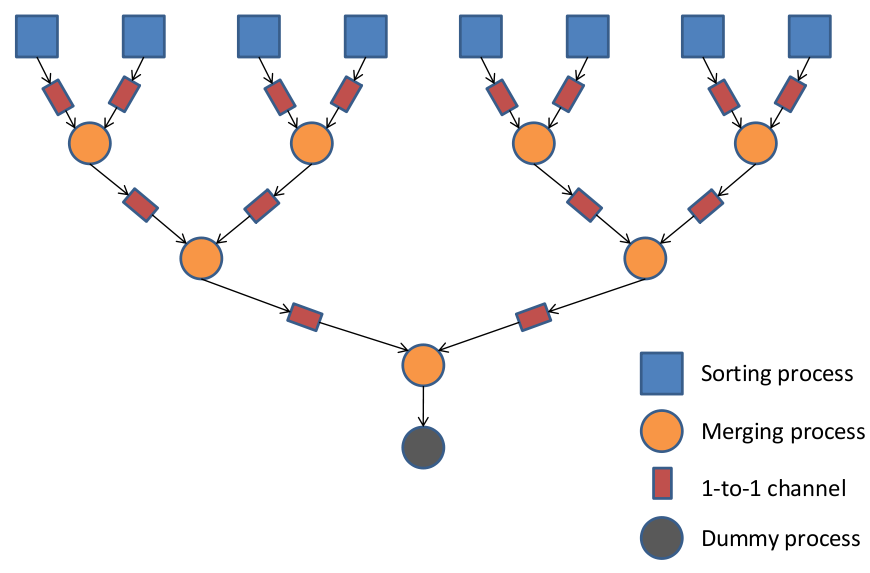
\includegraphics[width=\textwidth]{figures/mergesort}
\end{frame}

\begin{frame}[fragile]{MergeSort}
\begin{lstlisting}[basicstyle=\fontsize{7}{9}\selectfont\ttfamily]
public class MergeSort {
  // ...

  public static void main(String[] args) {
    // create extra receiver process for the final merging process
    One2OneChannel collectingChannel = Channel.one2one();
    DummyReceiverProcess dummyReceiverProcess = new DummyReceiverProcess(
        collectingChannel.in());

    // create thread hierarchy, connecting it to the extra receiver
    divide(1000, 32, collectingChannel.out());

    // put all JCSP processes in an array
    CSProcess[] allProcesses = new CSProcess[sortIndex + mergeIndex + 1];

    // Create sorting and merging processes including the extra 
    // receiver and put them into the array
    // ...

    Parallel parallel = new Parallel(allProcesses);
    parallel.run();
  }
}
\end{lstlisting}
\end{frame}

\begin{frame}[fragile]{\lstinline!divide()!}
\begin{lstlisting}[basicstyle=\fontsize{7}{9}\selectfont\ttfamily]
// recursively create sorting/merging processes and the interconnecting
// channels
private static void divide(int size, int noThreads, ChannelOutput out) {
  if (noThreads == 0) {
    SortingProcess sortingProcess = new SortingProcess(
        size, out);
    sortingProcesses.add(sortingProcess);
    sortIndex++;
  } else if (size >= 1) {
    One2OneChannel channel0 = Channel.one2one();
    One2OneChannel channel1 = Channel.one2one();
    MergingProcess mergingProcess = new MergingProcess(
        channel0.in(), channel1.in(), out);
    mergingProcesses.add(mergingProcess);
    mergeIndex++;

    int noThreadsLeft = noThreads - 1;

    divide(size / 2, noThreadsLeft / 2, channel0.out());
    divide(size - size / 2, noThreadsLeft - noThreadsLeft / 2, 
        channel1.out());
  }
}
\end{lstlisting}  
\end{frame}

\begin{frame}[fragile]{Sorting Process}
\begin{lstlisting}[basicstyle=\fontsize{7}{9}\selectfont\ttfamily]
public class SortingProcess implements CSProcess {
  private int[] chunk;
  private int chunkLength;
  private ChannelOutput next;

  public SortingProcess(int chunkLength, ChannelOutput next) { /* ... */ }

  public void run() {
    chunk = new int[chunkLength];
    Random r = new Random();
    for (int i = 0; i < chunkLength; i++)
      chunk[i] = r.nextInt(100);

    // sort chunk
    Arrays.sort(chunk);

    // write chunk size on output channel
    next.write(new Integer(chunkLength));
    // write chunk data, one by one, into output channel
    for (int i = 0; i < chunkLength; i++)
      next.write(new Integer(chunk[i]));
  }
}
\end{lstlisting}
\end{frame}

\begin{frame}[fragile]{Merging Process}
\begin{lstlisting}[basicstyle=\fontsize{7}{9}\selectfont\ttfamily]
public class MergingProcess implements CSProcess {
  private int[] chunk0, chunk1, sortedChunk;
  private int index0 = -1, index1 = -1, value;
  private AltingChannelInput prev0, prev1;
  private ChannelOutput next;

  public MergingProcess(AltingChannelInput prev0,
      AltingChannelInput prev1, ChannelOutput next) { /* ... */ }

  public void run() {
    Guard[] guards = { prev0, prev1 };
    Alternative alt = new Alternative(guards);

    while (true) {
      switch (alt.priSelect()) {
      case 0: // read from first input channel
        value = (Integer) prev0.read();
        // this is the first integer read, i.e., the chunk size
        if (index0 == -1) // chunk size
          chunk0 = new int[value];
        else // actual data
          chunk0[index0] = value;
        index0++;
        break;
\end{lstlisting}
\end{frame}

\begin{frame}[fragile]{Merging Process}
\begin{lstlisting}[basicstyle=\fontsize{7}{9}\selectfont\ttfamily]
      case 1: // read from second input channel
        value = (Integer) prev1.read();
        if (index1 == -1)
          chunk1 = new int[value];
        else
          chunk1[index1] = value;
        index1++;
        break;
      }
      // polling is finished if both chunks exist and are filled completely
      if (index0 > -1 && index1 > -1 && index0 == chunk0.length
          && index1 == chunk1.length)
        break;
    }

    sortedChunk = new int[chunk0.length + chunk1.length];
    // merge the two sorted chunks ...

    // write sorted chunk on output channel
    next.write(sortedChunk.length);
    for (i = 0; i < sortedChunk.length; i++)
      next.write(new Integer(sortedChunk[i]));
  }
}
\end{lstlisting}
\end{frame}

\begin{frame}[fragile]{Dummy Receiver Process}
\begin{lstlisting}[basicstyle=\fontsize{7}{9}\selectfont\ttfamily]
public class DummyReceiverProcess implements CSProcess {
  private ChannelInput prev;
  private int[] x;

  public DummyReceiverProcess(ChannelInput prev) { /* ... */ }

  public void run() {
    // read length of final, hopefully sorted, array
    int length = (Integer) prev.read();
    x = new int[length];
    // read final, hopefully sorted, array
    for (int i = 0; i < length; i++)
      x[i] = (Integer) prev.read();

    // check if the array is really sorted and print out result
    boolean isSorted = true;
    for (int i = 0; i < length - 1; i++)
      if (x[i] > x[i + 1]) {
        isSorted = false;
        break;
      }
    System.out.println("Succes = " + isSorted);
  }
}
\end{lstlisting}
\end{frame}


\section{Swing}

\begin{frame}{Outline}
  \tableofcontents[current]
\end{frame}

\begin{frame}{Swing}
  \begin{columns}[c]
    \begin{column}{0.55\textwidth}
      \begin{itemize}
      \item Swing is a platform-independent, Model-View-Controller GUI
        framework for Java
      \item Provides a native look and feel that emulates the look and
        feel of several platforms
      \item Supports a pluggable look and feel that allows applications to
        have a look and feel unrelated to the underlying platform
      \end{itemize}
    \end{column}
    \begin{column}{0.45\textwidth}
      \begin{center}
        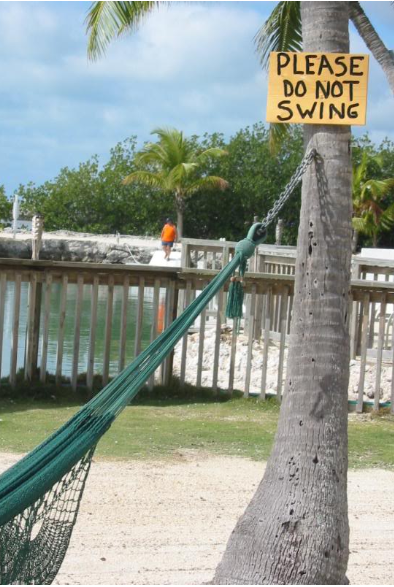
\includegraphics[width=\textwidth]{figures/do-not-swing}
      \end{center}
    \end{column}
  \end{columns}
\end{frame}

\begin{frame}[fragile]{Example: \lstinline{SimpleButton} (Initialization)}
\begin{lstlisting}[basicstyle=\fontsize{7}{9}\selectfont\ttfamily]
public class SimpleButton extends JPanel implements ActionListener {
  private final JButton computationButton, updateButton;
  private JTextField display;
  private final Counter counter = new Counter();

  private static void createAndShowGUI() {
    // Create and set up the window.
    JFrame frame = new JFrame("Simple Button with Action Listener");
    frame.setDefaultCloseOperation(JFrame.EXIT_ON_CLOSE);

    // Create and set up the content pane.
    SimpleButton newContentPane = new SimpleButton();
    newContentPane.setOpaque(true); // content panes must be opaque
    frame.setContentPane(newContentPane);

    // Display the window.
    frame.pack(); frame.setVisible(true);
  }

  public static void main(String[] args) {
    SwingUtilities.invokeLater(new Runnable() {
      public void run() { createAndShowGUI(); }
    });
  }
\end{lstlisting}
\end{frame}

\begin{frame}[fragile]{Example: \lstinline{SimpleButton} (Constructor)}
\begin{lstlisting}[basicstyle=\fontsize{7}{9}\selectfont\ttfamily]
  public SimpleButton() {
    computationButton = new JButton("Start computation");
    computationButton.addActionListener(this);
    computationButton.setActionCommand("compute");

    updateButton = new JButton("Update result");
    updateButton.addActionListener(this);
    updateButton.setActionCommand("update");

    display = new JTextField(20);
    display.setText(Integer.toString(0));
    display.setEditable(false);

    // Add Components to this container, using the default FlowLayout.
    add(computationButton);
    add(updateButton);
    add(display);
  }
\end{lstlisting}
\end{frame}

\begin{frame}[fragile]{Example: \lstinline{SimpleButton} (Action)}
\begin{lstlisting}[basicstyle=\fontsize{7}{9}\selectfont\ttfamily]
  /**
   * Starting the action triggers the computation
   */
  public void actionPerformed(ActionEvent e) {
    if ("compute".equals(e.getActionCommand())) {
      Thread[] t = new Thread[3];

      for (int i = 0; i < t.length; i++) {
        t[i] = new Thread(new ComputeTask(counter));
        t[i].start();
      }
    } else {
      // update command
      final int numActiveTasks = ComputeTask.getNumActiveTasks();
      if (numActiveTasks > 0) {
        display.setText(numActiveTasks
            + " are not finished, please wait");
      } else {
        display.setText(Integer.toString(counter.getValue()));
      }
    }
  }
}
\end{lstlisting}
\end{frame}

\begin{frame}[fragile]{Example: \lstinline{ComputeTask}}
\begin{lstlisting}[basicstyle=\fontsize{7}{9}\selectfont\ttfamily]
public class ComputeTask implements Runnable {
  private final Counter counter;
  private static int numActiveTasks = 0;

  public ComputeTask(Counter c) {
    this.counter = c;
  }

  public void run() {
    incrementNumActiveTasks();
    // sleep for a random time
    try {
      Thread.sleep((long) (Math.random() * 5000));
    } catch (InterruptedException e) {
      e.printStackTrace();
    }
    counter.increment();
    decrementNumActiveTasks();
  }

  // synchronized methods incrementNumActiveTasks, 
  // decrementNumActiveTasks, getNumActiveTasks
  // omitted...
}
\end{lstlisting}
\end{frame}

\begin{frame}[fragile]{Example: \lstinline{Counter}}
\begin{lstlisting}[basicstyle=\fontsize{7}{9}\selectfont\ttfamily]
public class Counter {
  private int val = 0;
  
  synchronized void increment() {
    val++;
  }
  
  synchronized int getValue() {
    return val;
  }
}
\end{lstlisting}

  \vspace{\stretch{1}}

  Alternative to writing your own thread-safe wrapper classes:
  \lstinline!AtomicInteger! (\url{http://java.sun.com/javase/6/docs/api/})
  \begin{itemize}
  \item \lstinline!incrementAndGet()!
  \item \lstinline!decrementAndGet()!
  \item \lstinline!get()!
  \end{itemize}
\end{frame}

\begin{frame}{Model-View-Controller}
  \begin{description}
  \item[Model:] Domain-specific representation of the data upon which
    the application operates, when a model changes its state, it
    notifies its associated views so they can be refreshed
  \item[View:] Renders the model into a form suitable for interaction,
    typically a user interface element, multiple views can exist for a
    single model for different purposes
  \item[Controller:] Receives input and initiates a response by making
    calls on model objects
  \end{description}
\end{frame}

\begin{frame}{Model-View-Controller: Sun}
  \begin{center}
    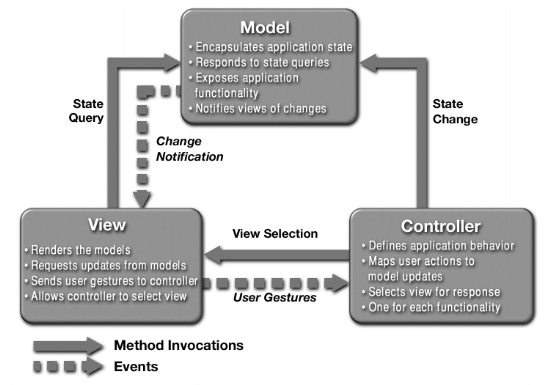
\includegraphics[scale=0.4]{figures/mvc} \\
    \tiny{Source: \url{http://java.sun.com/blueprints/patterns/MVC-detailed.html}}
  \end{center}
\end{frame}

\begin{frame}{Model-View-Controller: Ruby on Rails}
  \begin{center}
    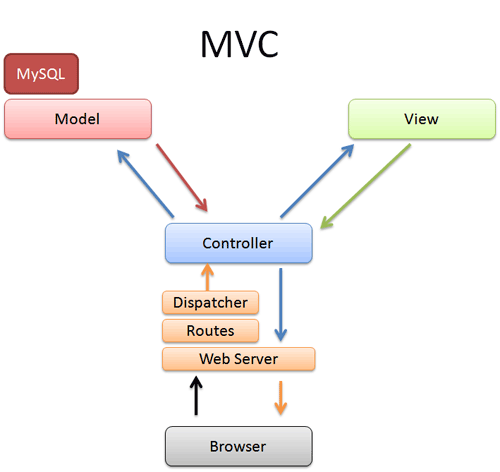
\includegraphics[scale=0.4]{figures/mvc-rails} \\
    \tiny{Source: \url{http://betterexplained.com/articles/intermediate-rails}}
  \end{center}
\end{frame}

\begin{frame}{Tutorials}
  \begin{itemize}
  \item Creating a GUI With JFC/Swing:\\
    \url{http://java.sun.com/docs/books/tutorial/uiswing/}
  \item Using Swing Components:\\
    \url{http://java.sun.com/docs/books/tutorial/uiswing/components/index.html}
  \item Ein (sehr) kleines Swing Tutorial:\\
    \url{http://www.mm.informatik.tu-darmstadt.de/courses/helpdesk/swing.html}
  \end{itemize}
\end{frame}


\section{Game of Life}

\begin{frame}{Outline}
  \tableofcontents[current]
\end{frame}

\begin{frame}{Conway's Game of Life}
  \begin{columns}[c]
    \begin{column}{0.45\textwidth}
      \begin{itemize}
      \item Implement ``Game of Life'' with GUI based on Swing
      \item Model-View-Controller Pattern
      \item You can use the given code skeleton
      \item Let's see an example
      \end{itemize}
    \end{column}
    \begin{column}{0.55\textwidth}
      \begin{center}
        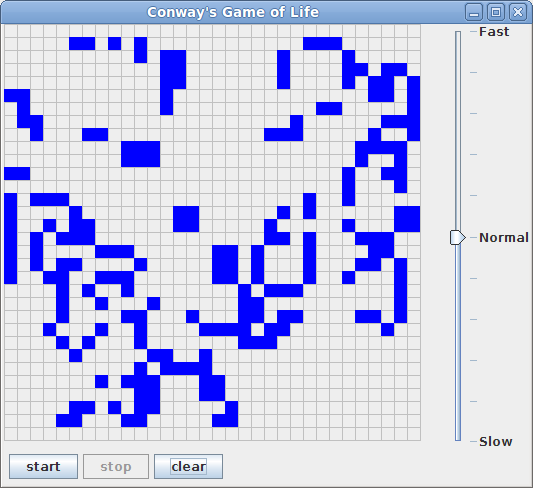
\includegraphics[width=\textwidth]{figures/gol}
      \end{center}
    \end{column}
  \end{columns}

  \vspace{\stretch{1}}

  See \url{http://en.wikipedia.org/wiki/Conway's_Game_of_Life}
\end{frame}

\begin{frame}{Universe}
  \begin{itemize}
  \item The universe of the Game of Life is an infinite
    two-dimensional orthogonal grid of square cells
    \begin{itemize}
    \item Our implementation uses a finite grid
    \end{itemize}
  \item Each cell is in one of two possible states:
    \begin{itemize}
    \item live
    \item dead
    \end{itemize}
  \item Every cell interacts with its eight neighbors, which are the
    cells that are directly
    \begin{itemize}
    \item horizontally
    \item vertically
    \item diagonally
    \end{itemize}
    adjacent
  \end{itemize}
\end{frame}

\begin{frame}{Rules}
  At each step in time, the following transitions occur:

  \vspace{\stretch{1}}

  \begin{enumerate}
  \item Any live cell with fewer than two live neighbours dies, as if
    caused by underpopulation
  \item Any live cell with more than three live neighbours dies, as if
    by overcrowding
  \item Any live cell with two or three live neighbours lives on to
    the next generation
  \item Any dead cell with exactly three live neighbours becomes a
    live cell
  \end{enumerate}  
\end{frame}


\section*{Outro}

\begin{frame}{Summary}
  \begin{itemize}
  \item Monitors don't provide any fairness
    \begin{itemize}
    \item Could use \lstinline!Semaphore(int permits, boolean fair)!
      for example
    \end{itemize}
  \item CSP provides synchronous communication
    \begin{itemize}
    \item Synchronous communication implies that sender and receiver
      must ``meet'' to exchange data $\rightarrow$ if one of them does
      not reach the correct communication operations, the other one
      waits for ever
    \end{itemize}
  \item MergeSort implementation using JCSP
  \item Try to separate Swing related code from your model
  \item Conway's Game of Life
  \end{itemize}
\end{frame}

\end{document}
